% D.20 等腰梯形 ABCD：AD=4，BC=10，AB=CD=5（高=4）
\documentclass[tikz,border=4pt]{standalone}
\usepackage{ctex}
\usepackage{amsmath}
\usetikzlibrary{calc}
\begin{document}
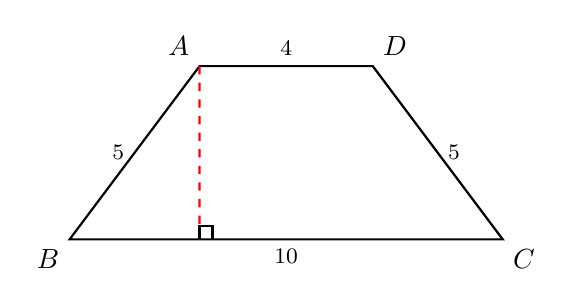
\begin{tikzpicture}[scale=0.55, thick]
  \coordinate (B) at (0, 0);
  \coordinate (C) at (10, 0);
  \coordinate (A) at (3, 4);
  \coordinate (D) at (7, 4);

  \draw (A) -- (B) -- (C) -- (D) -- cycle;
  % 高
  \draw[red, dashed] (A) -- (3, 0);
  \draw (3,0) -- (3,0.3) -- (3.3,0.3) -- (3.3,0);

  \node[above left]  at (A) {$A$};
  \node[below left]  at (B) {$B$};
  \node[below right] at (C) {$C$};
  \node[above right] at (D) {$D$};

  \node[above] at ($(A)!0.5!(D)$) {\footnotesize $4$};
  \node[below] at ($(B)!0.5!(C)$) {\footnotesize $10$};
  \node[left]  at ($(A)!0.5!(B)$) {\footnotesize $5$};
  \node[right] at ($(C)!0.5!(D)$) {\footnotesize $5$};
\end{tikzpicture}
\end{document}
